\chapter{Results}

\section{Hardware testing}

A total of 40 FLX-182-1B cards, in 3 different batches, were subjected hardware validation and testing. During this process, 10 cards were found to be non-functional due to a range of issues, including component failures and configuration errors. Through the aformentioned diagnostics and interventions, 8 of the faulty cards were fully or partially recovered and restored to operational status.\\
All the recovered cards are now delivered to the institutes and functioning properly.

\section{Performance measurements: netio3}
\label{sec:netio3-perf}
The network performance evaluation focused on two key parameters: Throughput and \ac{RTT}. The experiments were conducted in a controlled testbed environment using servers connected via a 200 Gbit/s Ethernet link. The hardware specifications of the servers are detailed below:

\clearpage
\begin{lstlisting}[caption={Network interface information}, label={lst:network}]
[mshehu@pc-tbed-felix-15 ~]$ lspci | grep -E -i --color 'network|ethernet'
41:00.0 Ethernet controller: Mellanox Technologies MT2910 Family [ConnectX-7]
41:00.1 Ethernet controller: Mellanox Technologies MT2910 Family [ConnectX-7]
81:00.0 Ethernet controller: Intel Corporation Ethernet Controller X550 (rev 01)
81:00.1 Ethernet controller: Intel Corporation Ethernet Controller X550 (rev 01)
\end{lstlisting}

\begin{lstlisting}[caption={CPU information}, label={lst:cpu}, float=htbp]
[mshehu@pc-tbed-felix-15 ~]$ lscpu
Architecture:             x86_64
  CPU op-mode(s):         32-bit, 64-bit
  Address sizes:          52 bits physical, 57 bits virtual
  Byte Order:             Little Endian
CPU(s):                   64
  On-line CPU(s) list:    0-63
Vendor ID:                AuthenticAMD
  Model name:             AMD EPYC 9354P 32-Core Processor
    CPU family:           25
    Model:                17
    Thread(s) per core:   2
    Core(s) per socket:   32
    CPU max MHz:          3799.0720
    CPU min MHz:          1500.0000
\end{lstlisting}

\clearpage
\begin{lstlisting}[caption={Memory information}, label={lst:memory}]
[mshehu@pc-tbed-felix-15 ~]$ lsmem
RANGE                                 SIZE  STATE REMOVABLE BLOCK
0x0000000000000000-0x000000187fffffff  98G online       yes  0-48
\end{lstlisting}

The receiving machine was equipped with an older FLX-712 card, while the sending machine utilized the new FLX-182-1B prototype developed for Phase II. This emulates the \texttt{felix-tohost} direction. The statics have been collected from the sending part; the reason was because the sending part interrupts the connection, and the statistics collection could be stopped at the same time.

The throughput tests were conducted using the two \textit{netio3-backends} LIBFABRIC-RDMA and ASYNCMSG-TCP. To manage the high number of tests, an Ansible \cite{ansible} playbook was developed. The output of the playbook was processed using a custom Python script, which also generated the graphs using the Matplotlib \cite{matplotlib} library. The tests involved varying the buffer size --- ranging from 1 KB to 64 KB  (in ATLAS production are used buffers of 64 KB) --- and the number of buffers. The same buffer size and number of buffers were used for both the sender and receiver. 

The sender transmits buffers sequentially, employing a polling mechanism to determine when the next buffer could be sent. The receiver, in turn, simply ackowledges and discards the incoming messages without further processing, as the primary objective was to measure throughput. A total of 70 combinations of buffer sizes and counts were tested for LIBFABRIC-RDMA, while only 28 combinations were evaluated for ASYNCMSG-TCP due to diminishing returns observed in preliminary tests.

\subsection{Analysis}

Figures \ref{fig:1kb-buffer-throughput} and \ref{fig:64kb-buffer-throughput} shows the measurements for the two extreme cases: a 1 KB buffer and a 64 KB buffer.

\begin{figure}[htbp]
\centering
\begin{subfigure}[b]{0.7\textwidth}
    \centering
    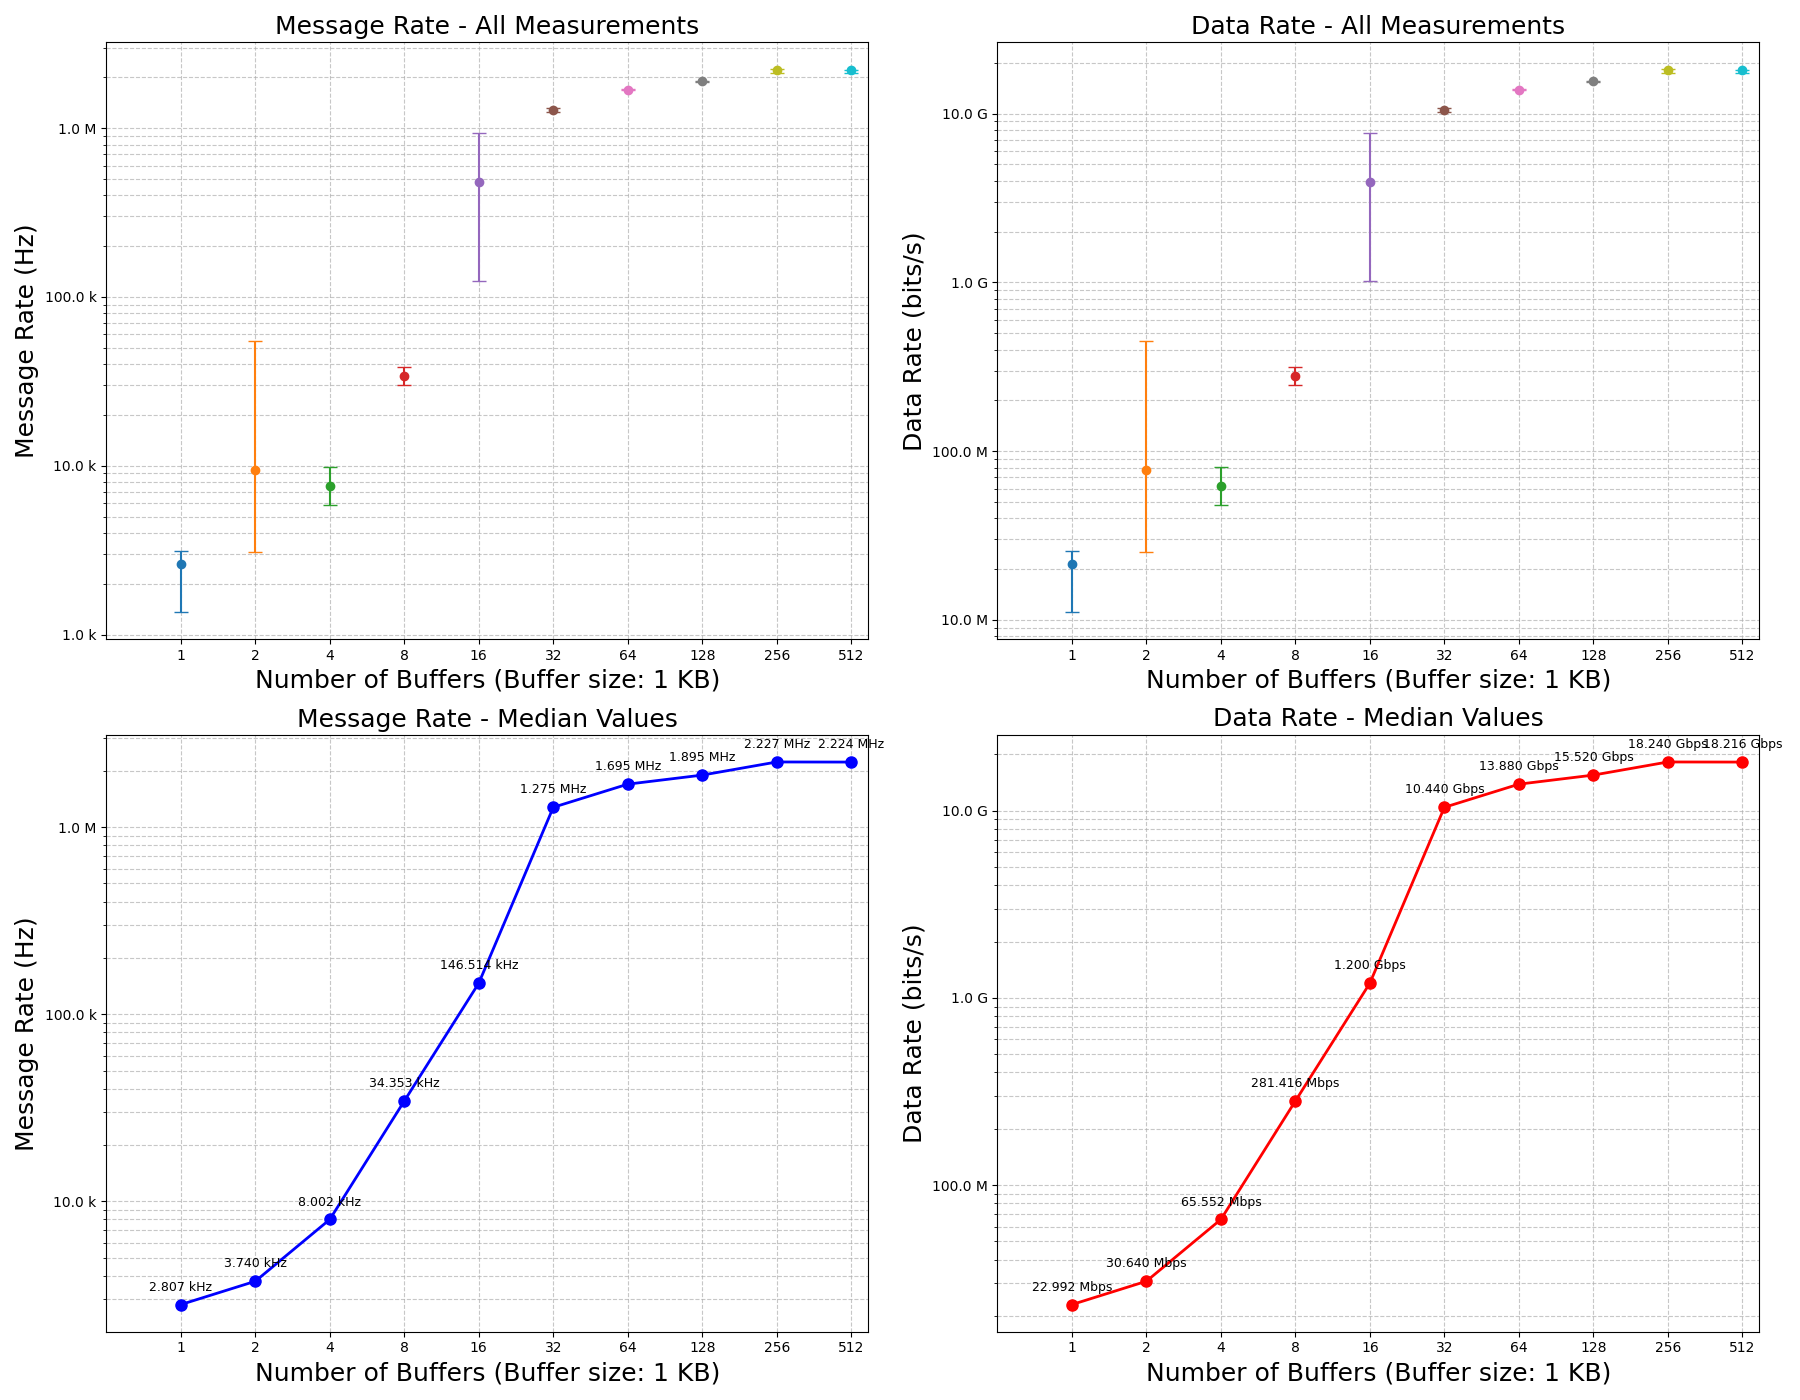
\includegraphics[width=\textwidth]{images/results/libfabric_throughput_analysis_1K.png}
    \caption[Network performance with a 1 KB buffer]{Network performance with a 1 KB buffer. \textbf{Left:} message frequency, \textbf{Right:} Data Throughput. \textbf{Top:} plots with error ranges, \textbf{Bottom:} median values.}
    \label{fig:1kb-buffer-throughput}
\end{subfigure}
\vspace{0.2cm}
\begin{subfigure}[b]{0.7\textwidth}
    \centering
    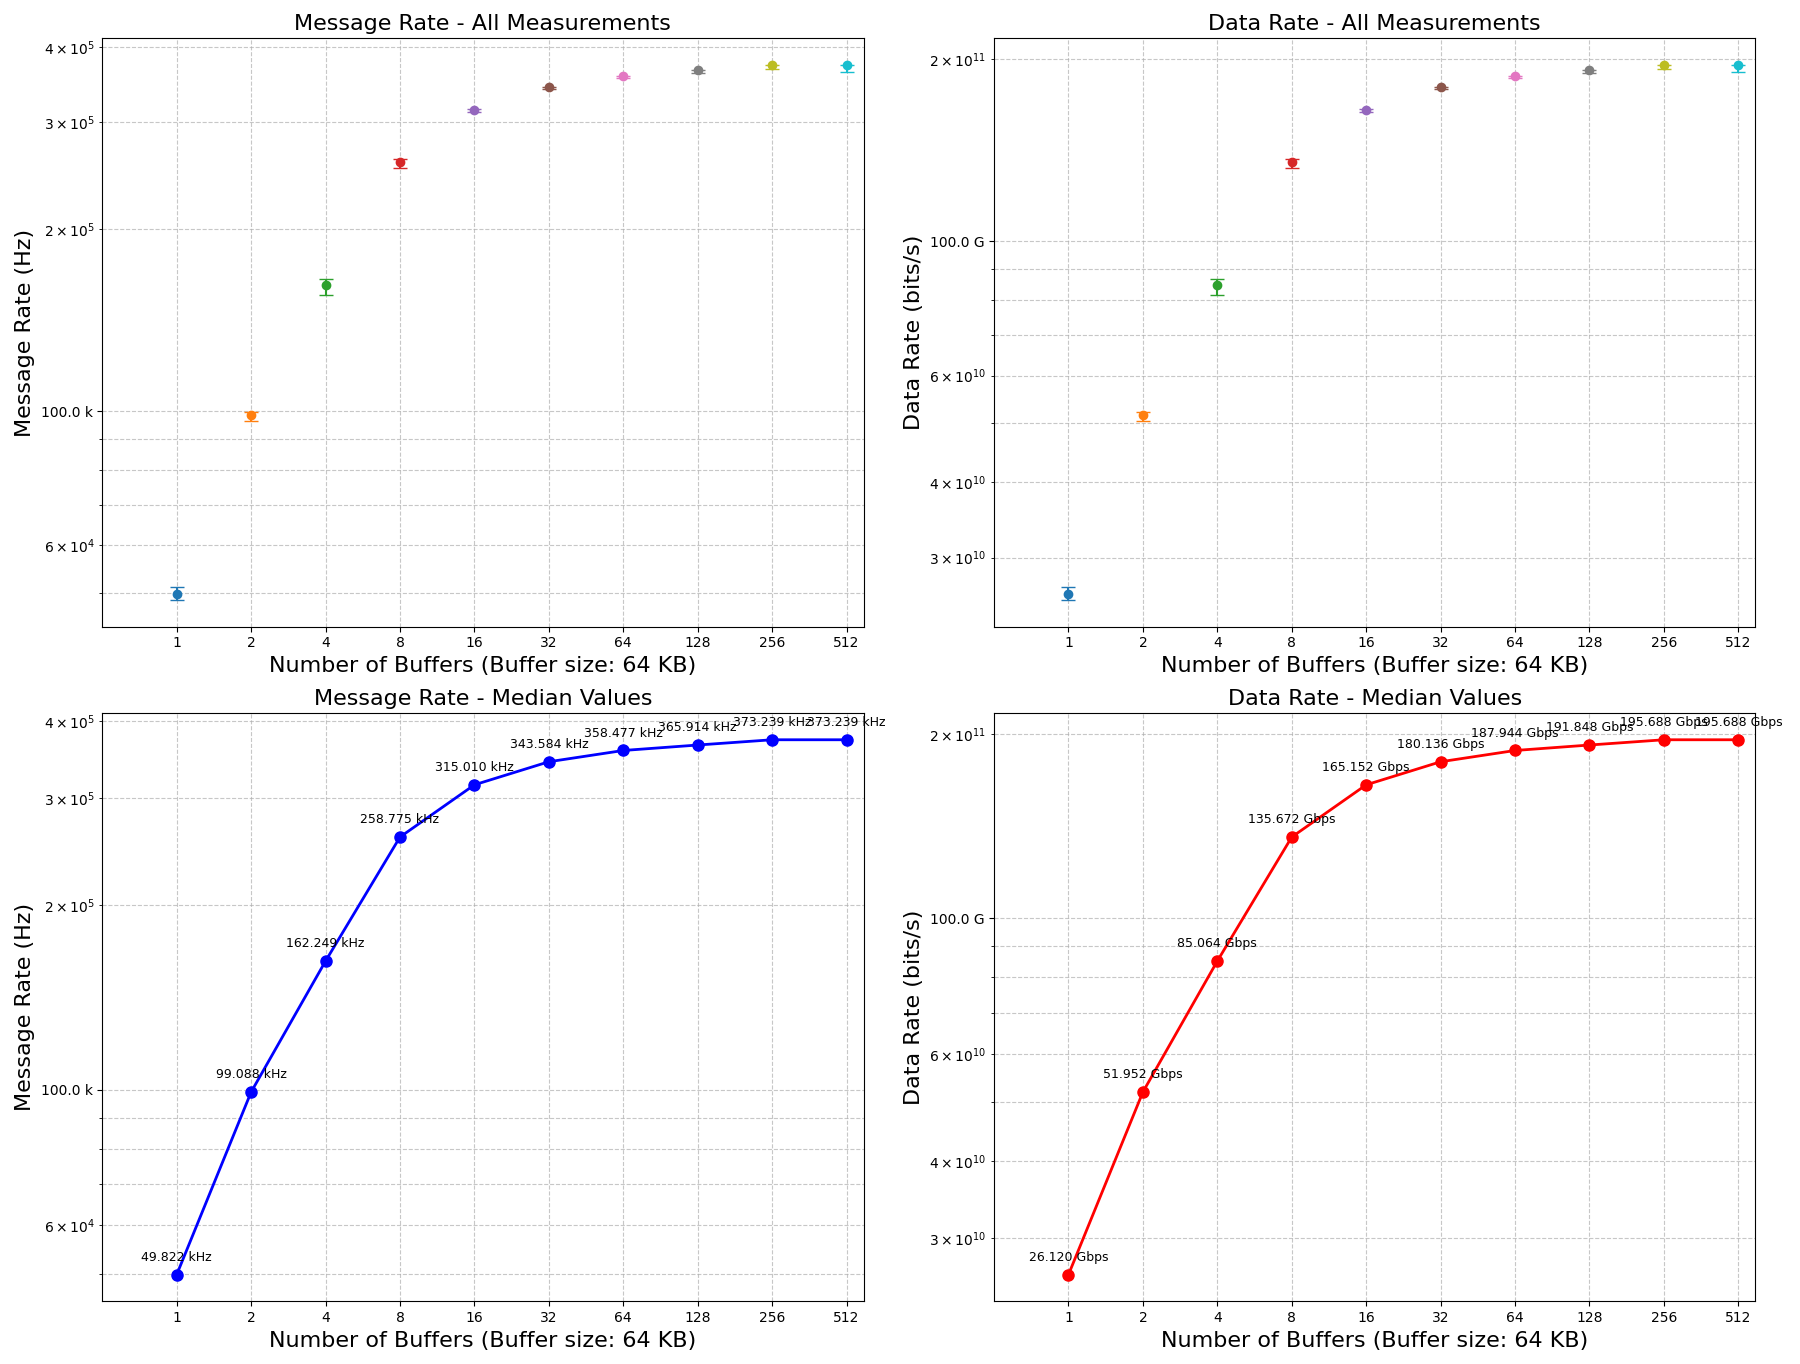
\includegraphics[width=\textwidth]{images/results/libfabric_throughput_analysis_64K.png}
    \caption[Network performance with a 64 KB buffer]{Network performance with a 64 KB buffer. \textbf{Left:} message frequency, \textbf{Right:} Data Throughput. \textbf{Top:} plots with error ranges, \textbf{Bottom:} median values.}
    \label{fig:64kb-buffer-throughput}
\end{subfigure}
\caption[Throughput comparison of 1KB and 64KB buffer]{The error rate of the smaller 1KB buffers is relatively high, while for the 64KB buffers the effect is much more contained.}
\label{fig:throughput-of-the-extremes-1K-64K}
\end{figure}

The results indicate that smaller buffers (e.g., 1 KB) exhibit higher error rates due to the overhead associated with connection establishment, which is significant relative to the transmission time for small messages. In contrast, larger buffers (e.g., 64 KB) exhibit a small variance, as the connection overhead becomes negligible compared to the transmission time.

To mitigate the impact of these variations (especially for smaller buffers), the median throughput was used for comparison.

Figure \ref{fig:libfabric-mean-throughput-comparison} presents the throughput comparison for LIBFABRIC-RDMA across all buffer sizes. The results highlight that buffers smaller than 8 KB and a fewer number of buffers than 16 should be avoided. For larger buffers, the behavior aligns with expectations. 
An interesting observation can be made about smaller buffers achieving the expected rate.

\begin{figure}[htbp]
\centering
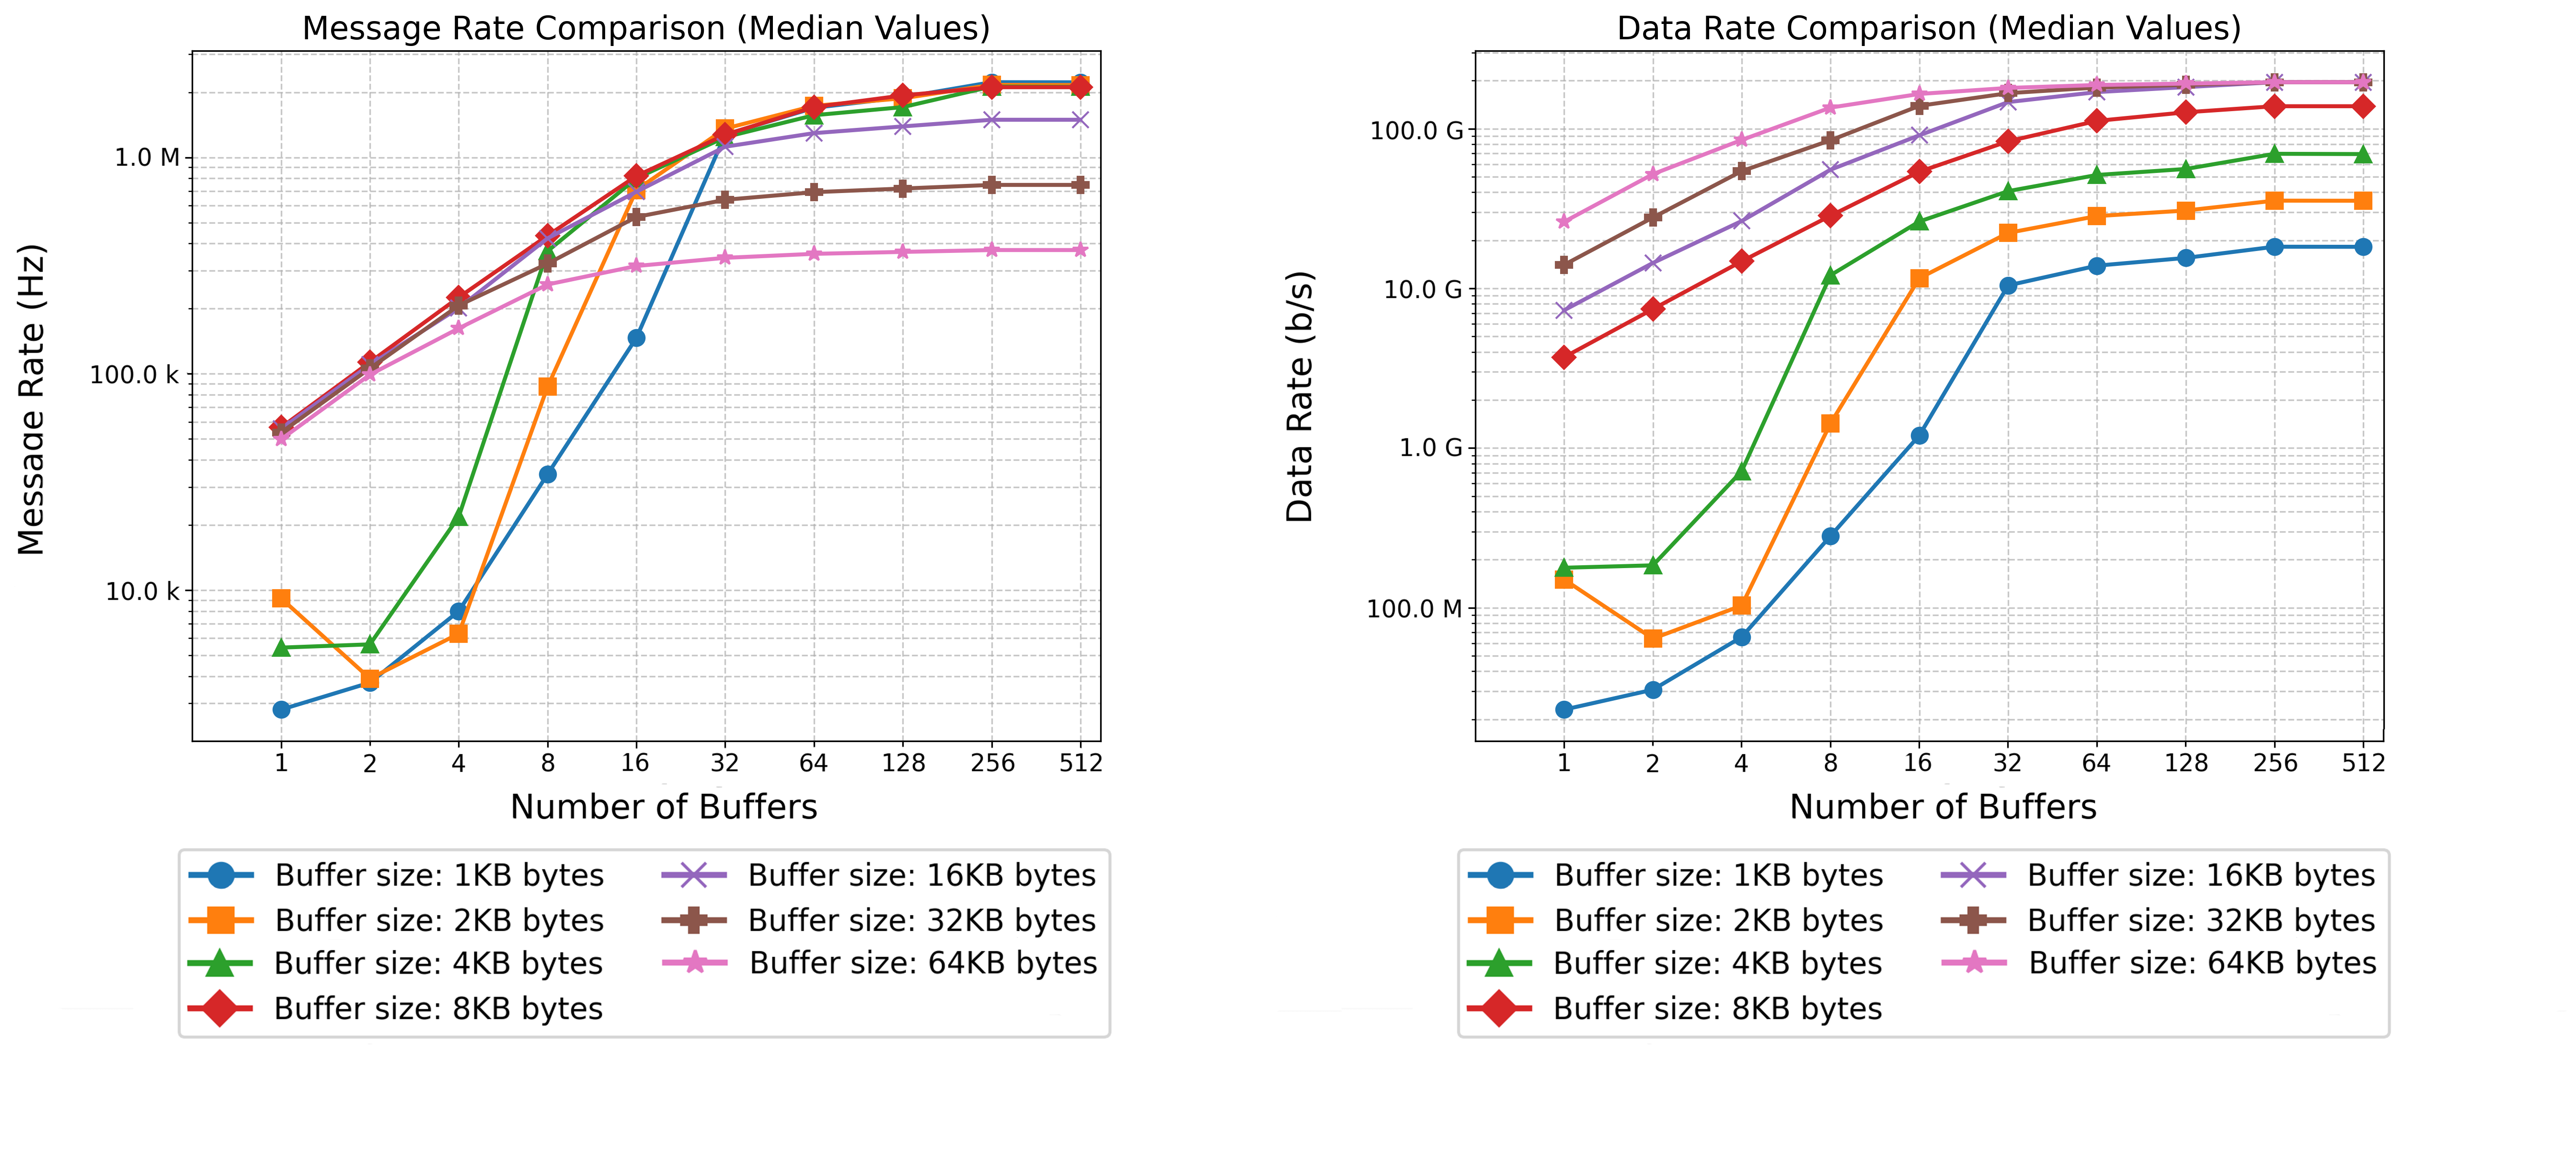
\includegraphics[width=\textwidth]{images/results/libfabric_performance_comparison.png}
\caption[Throughput comparison for LIBFABRIC-RDMA across all buffer sizes]{Throughput comparison for LIBFABRIC-RDMA across all buffer sizes. Left: frequency; Right: throughput.}
\label{fig:libfabric-mean-throughput-comparison}
\end{figure}

The throughput results also demonstrate that the 200 Gbps bandwidth is quickly saturated when using larger buffers. Notably, the network library can handle 64 KB buffers at 100 MHz, meeting the requirements for Phase II production.

For ASYNCMSG-TCP, the results (Figure \ref{fig:tcp-mean-throughput-comparison}) reveal that smaller buffers consistently achieve higher rates, regardless of the number of buffers. The throughput is significantly lower than LIBFABRIC-RDMA, with rates ranging from 70 to 90 kHz and a maximum throughput below 10 Gbps. This performance disparity shows once again that LIBFABRIC-RDMA can handle larger amount of data compared to ASYNCMSG-TCP.

\begin{figure}[htbp]
\centering
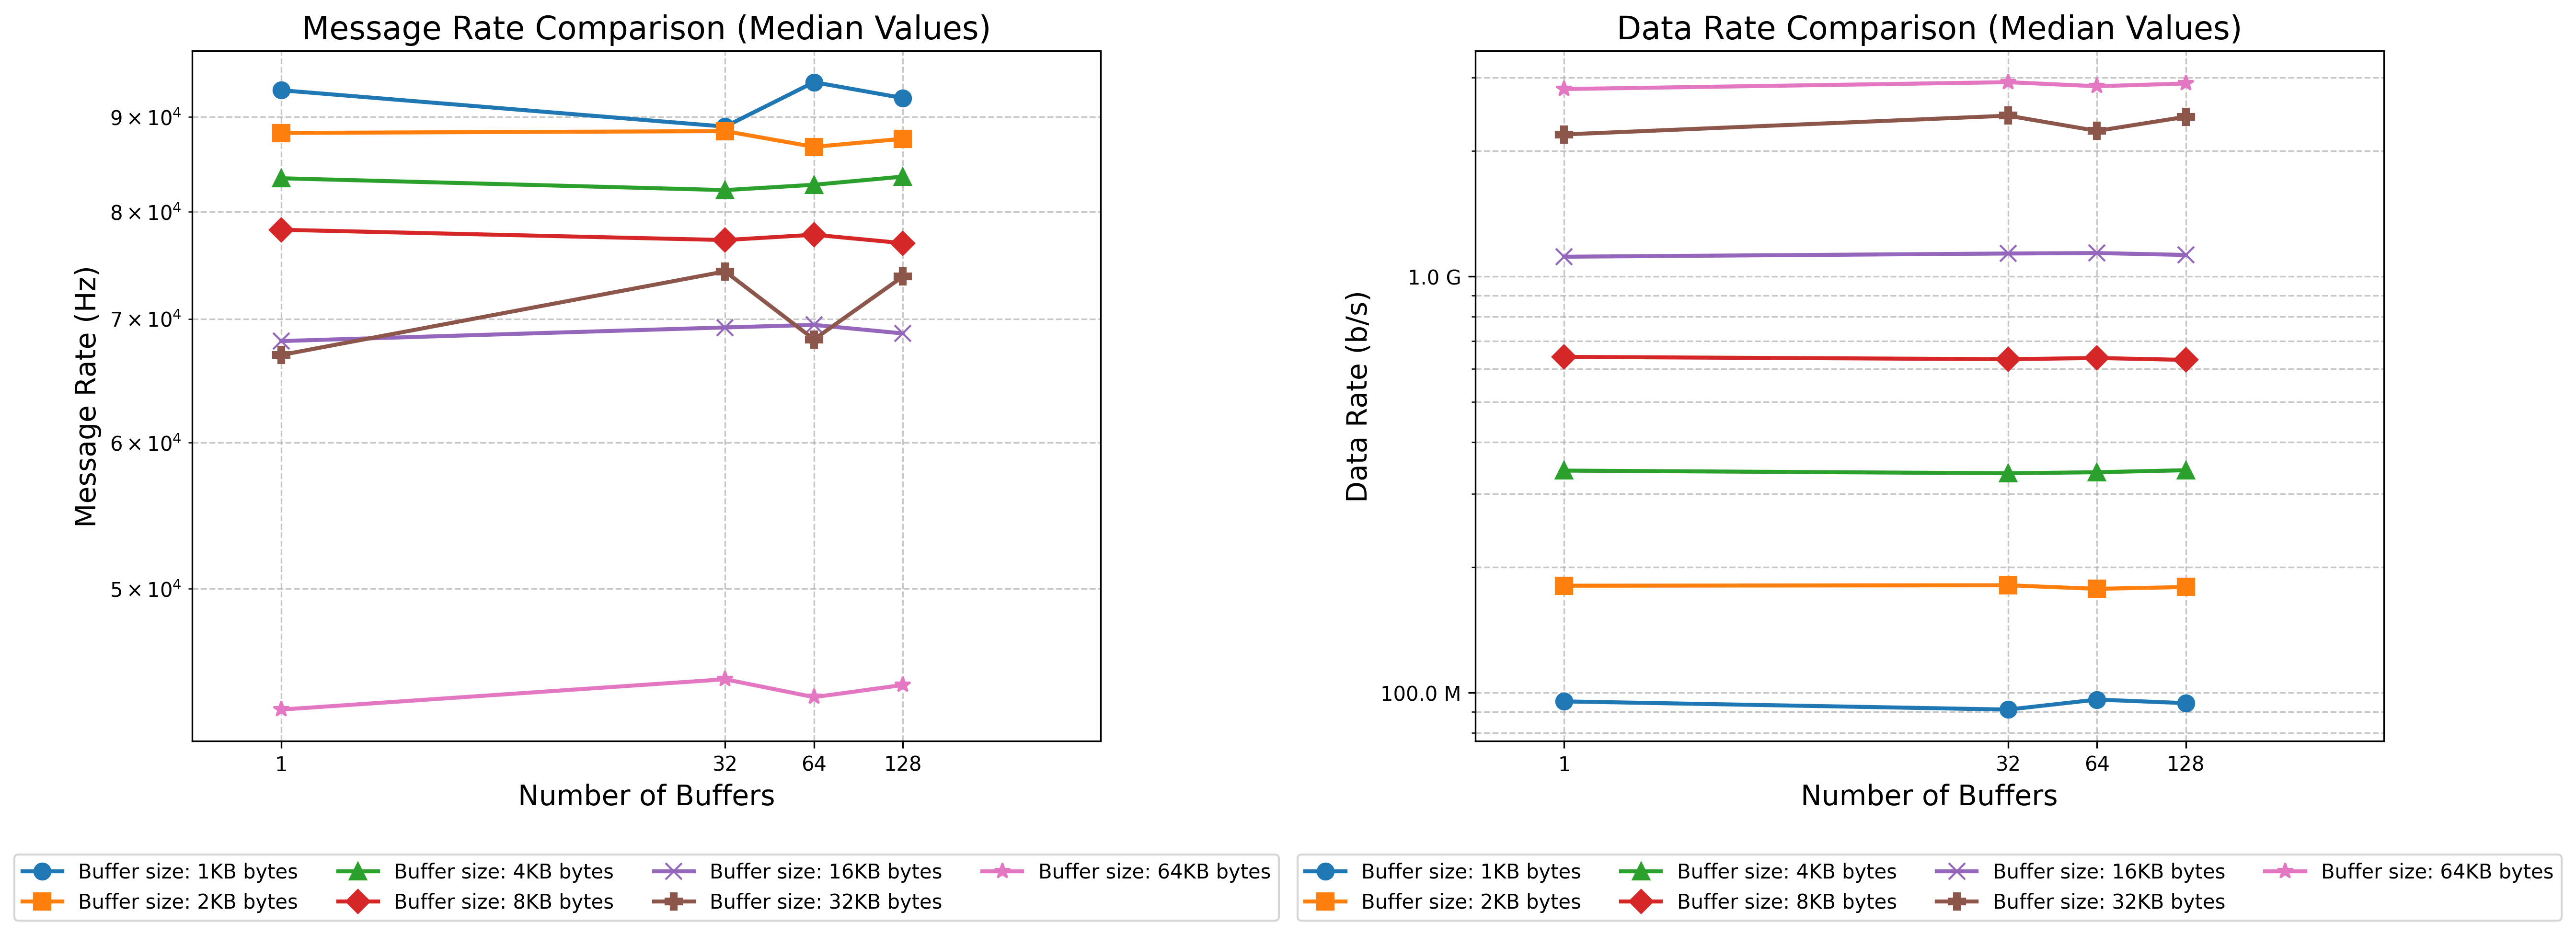
\includegraphics[width=\textwidth]{images/results/tcp_performance_comparison.png}
\caption[Throughput comparison for ASYNCMSG-TCP across all buffer sizes]{Throughput comparison for ASYNCMSG-TCP across all buffer sizes. Left: frequency; Right: throughput.}
\label{fig:tcp-mean-throughput-comparison}
\end{figure}

The decision to limit the number of buffers and sizes tested for ASYNCMSG-TCP was based on the observed saturation of bandwidth for LIBFABRIC-RDMA and the lack of performance improvement for ASYNCMSG-TCP with larger buffers. These findings conclusively demonstrate that LIBFABRIC-RDMA outperforms ASYNCMSG-TCP in terms of data throughput.

Given those results, why is TCP included as an option? One of the reasons is that it is less computationally demanding than \acs{RDMA}, so it is a better choice where the computing power is limited (L1 Calorimeter for example). The other reason derives from internal needs of \acs{ATLAS} and how its monitoring works. In order to monitor the entirety of \acs{ATLAS}' \acl{FE} electronics many elinks need to be used, in that case using LIBFABRIC-RDMA would require creating a \acs{DMA} buffer for each of them, plus sometimes the network library is used to send configurations to \acs{FE} electronics, meaning that the buffers need to be big enough for such scenarios. It comes by itself that the amount of memory needed is very large, and that memory would not be used efficiently, also the use case of the monitoring does not require high performance, thus ASYNCMSG-TCP is ideal.

\clearpage
\section{Performance measurements: felix-tohost}

\texttt{felix-tohost} represents the data direction from the Detectors to the T-DAQ infrastructure and between. The measurements that follow were conducted on the same device and host used for the \texttt{netio3} performance evaluation (Section~\ref{sec:netio3-perf}). 
Figure~\ref{fig:tbed-setup} below illustrates the setup for the test.\\
\emph{pc-tbed-felix-15} mounts the currently used in production \emph{FLX-712} with the \emph{F-EMU} firmware, which is used to emulate data in the FULLMODE format; that data will be written inside \acs{DMA} buffers on the other machine through \acs{E-link}s. It can be configured which \acs{E-link} writes in which \acs{DMA} buffer using the \emph{elinkconfig} tool. In the context of this test, all the 12 links have been used, specifically 3 links per \acs{DMA} buffer. 
On the same machine runs \emph{felix-test-swrod}, which is a software that subscribes to the \acs{E-link}s through \texttt{felix-tohost}, which in turn publishes the data when available.
On \emph{pc-tbed-felix-14} is mounted an \emph{FLX-182-1B} card, which is a prototype for the Phase II upgrade, with FULLMODE firmware. On the machine runs \texttt{felix-tohost}, which, as mentioned, will publish the data received from the emulator to \emph{felix-test-swrod} and will post the monitoring data so that a Prometheus instance running on Docker on my local machine could scrape it, and in turn Grafana could query Prometheus for the data scraped and create the Dashboard seen in Figure~\ref{fig:tohost-perf}. On \emph{pc-tbed-felix-14}, there is also the \acl{TTC} emulator that gives the pace to the FULLMODE emulator; in this test, the emulator trigger signals were set at 1 MHz.\\
For what concerns the \emph{netio3} network library, LIBFABRIC-RDMA was used.\\
The test consisted of sending data through all 12 links distributed across 4 \acs{DMA} buffers (3 links per \acs{DMA} buffer) at a steady 1 MHz rate, but changing the \emph{chunk} size.\\
As a reminder, in FULL mode, each link is not subdivided into \acs{E-link}s.

\begin{figure}[htbp]
\centering
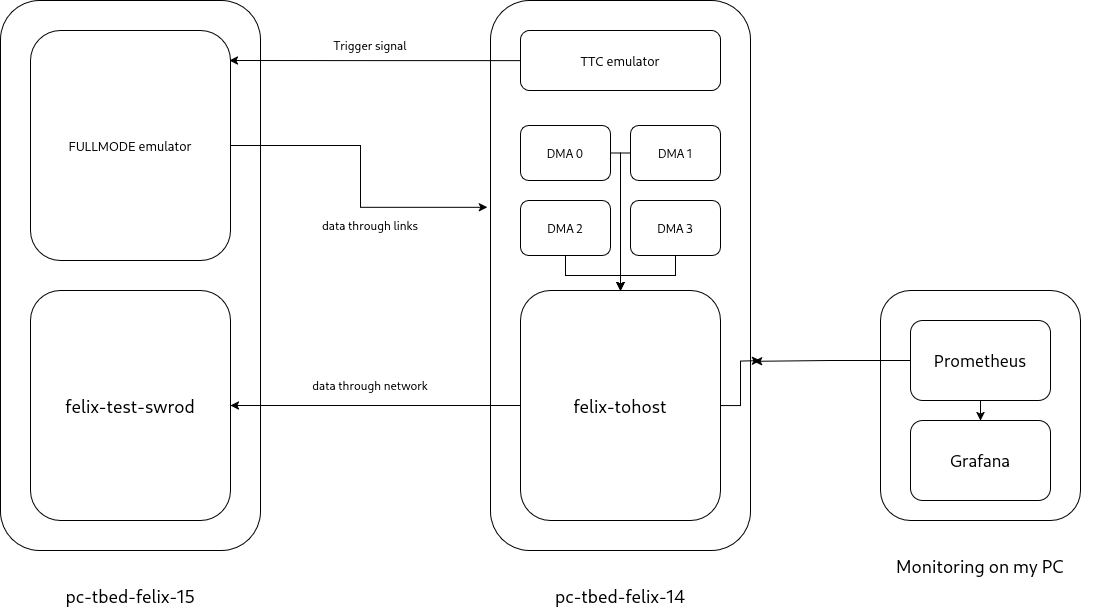
\includegraphics[width=\textwidth]{images/results/tohost-tbed-setup.png}
\caption[Testbed configuration]{Testbed configuration. F-EMU firmware is installed on the felix-15 machine, felix-tohost is running on the felix-14 machine which also sends the monitoring data to Prometheus.}
\label{fig:tbed-setup}
\end{figure}

The monitoring system described in Section~\ref{sec:felix_monitoring} was employed to record the performance evaluation, in particular the Prometheus-Grafana solution. The test was conducted by gradually increasing the \emph{chunk} size while maintaining a steady rate of 1 MHz (what is the requirement for Phase II). This behavior is illustrated in the dashboard window titled "Average Chunk Size" (Image~\ref{fig:tohost-perf}), where the average chunk size ramps, with incremental steps, from 16 bytes to 2 KB. Starting at a chunk size of 1 KB, by looking at the \emph{E-link Chunk Rate} graph it appears that performance issues begin to arise.\\
What in reality is shown in the image is not a performance issue, but it is the reach of the physiological limit of FULL mode. To recall, the Subsection~\ref{subsec:felix-fullmode} explains that FULL mode has a maximum theoretical throughput of about 7.68 Gbps per link (after encoding, which is our case), and in the graph it is shown that the \acs{DMA} buffers are not getting filled up (\emph{Free Space in DMA Buffer} graph), there is no backpressure in the network (\emph{Network Resources} graph) and the chunks are not being truncated (\emph{Chunks Truncated} graphs). at a rate of 1MHz, sending 1KB of data per chunk means that the throughput is about 8.2 Gbps, and at 2KB it is about 16.4 Gbps, which is above the maximum throughput of the link, thus the link chunk rate diminishes untill reaching 7.68 Gbps throughput.\\ 
To recap, in figure~\ref{fig:tohost-perf} is shown that \texttt{felix-tohost} and the card \texttt{FLX-182-1B} can handle without signs of distress data rates that reach the technological limit of FULL mode.

\begin{figure}[htbp]
\centering
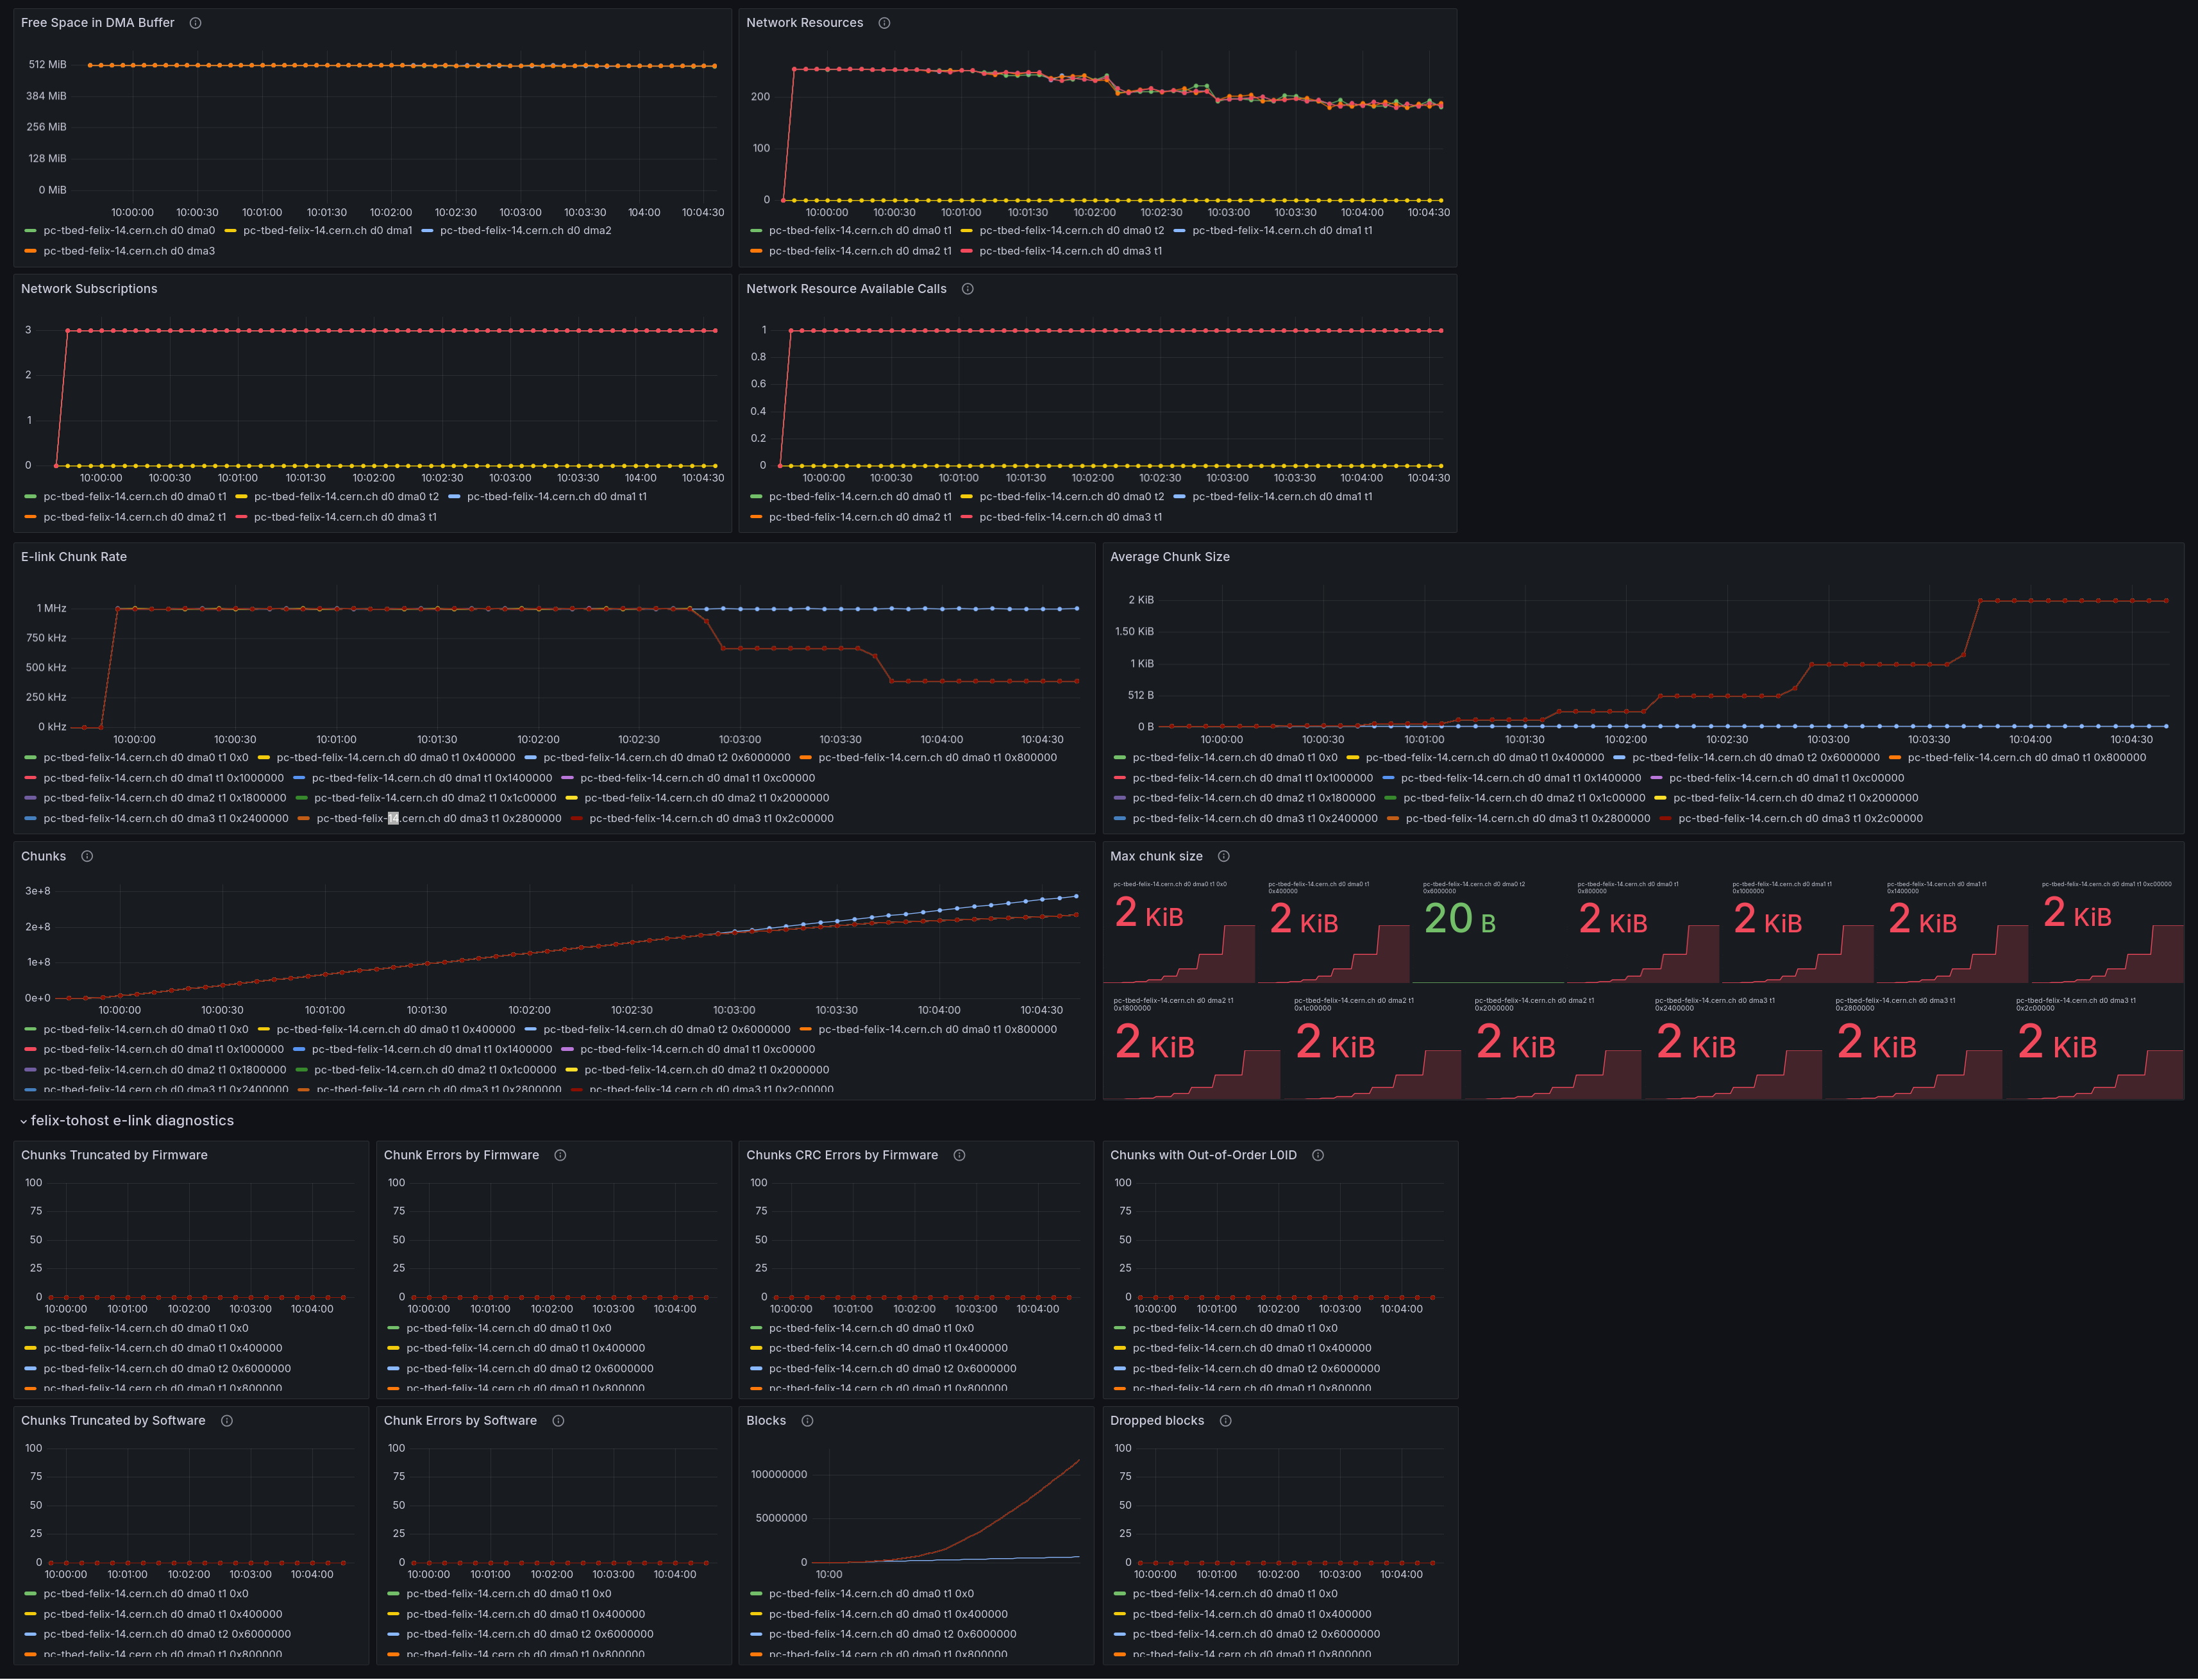
\includegraphics[width=\textwidth]{images/results/tohost-perf.png}
\caption{Grafana monitoring: stress test at 1 MHz rate up to 2 KB chunks.}
\label{fig:tohost-perf}
\end{figure}

Figure~\ref{fig:cpu-usage} illustrates the CPU usage per chunk size. The percentage value represents the average CPU usage over a 30-second period. Given that the host machine has 64 CPU cores, the results demonstrate that \emph{felix-tohost} is not very resource-intensive.

\begin{figure}[htbp]
\centering
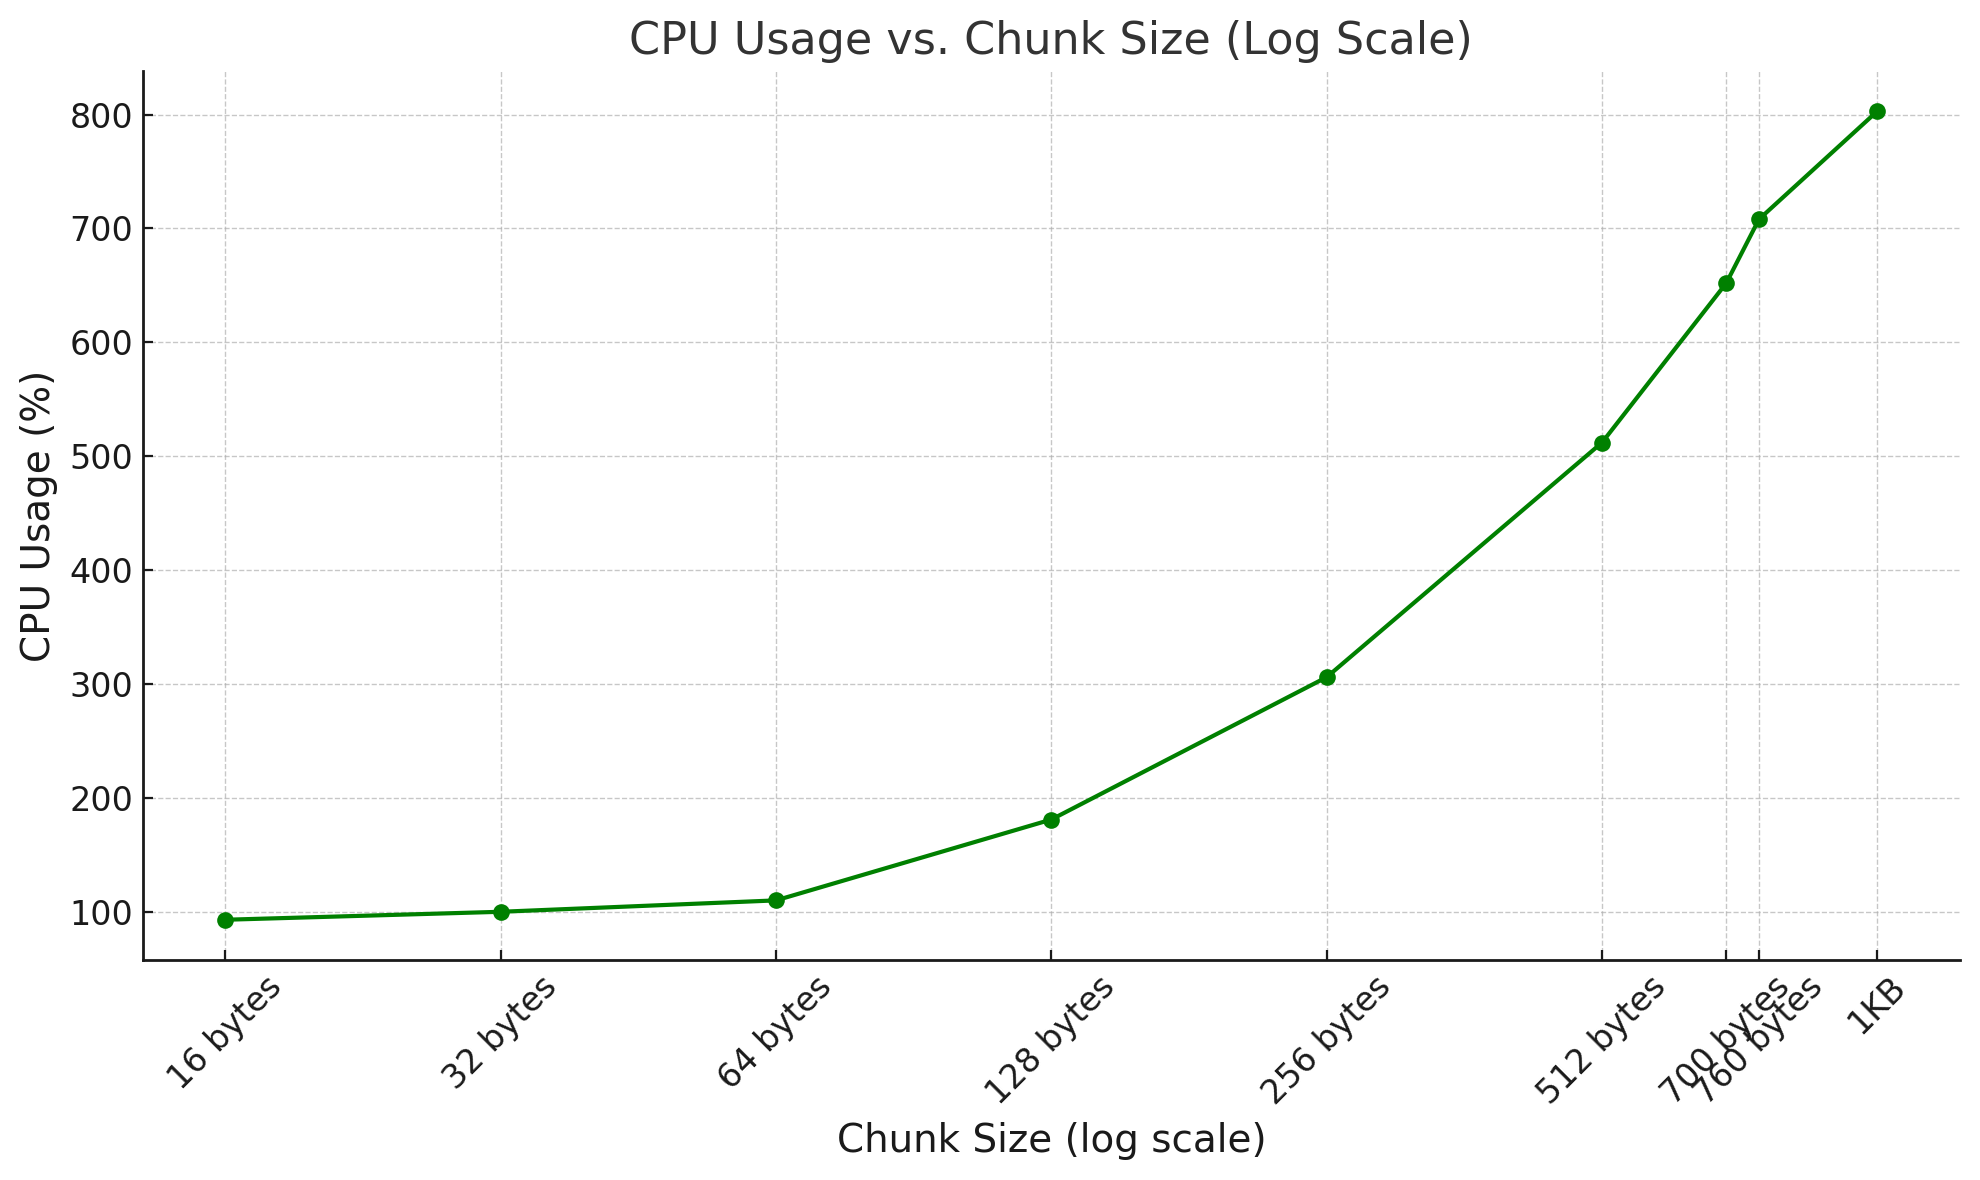
\includegraphics[width=\textwidth]{images/results/cpu-usage-chunk-size-1MHz.png}
\caption[CPU usage per chunk size at 1 MHz]{CPU usage per chunk size at 1 MHz. 100\% corresponds to one physical CPU core.}
\label{fig:cpu-usage}
\end{figure}

The execution of \texttt{felix-tohost} was analyzed using \texttt{perf}, and from the output a FlameGraph \cite{flamegraph} was generated (Figure~\ref{fig:felix-tohost-flamegraph}). The FlameGraph, an interactive \emph{svg} file viewable in a web browser, shows that a significant portion of the execution time is spent on functions such as \emph{decode\_subchunk\_headers}, \emph{post\_subchunk}, and \emph{check\_block\_integrity}, as well as chunk-copying operations. This flamegraph shows hotpost areas in the code that can potentially be optimized, serving as a starting point for future developments (see Subsection~\ref{subsec:felix-tohost-improvement}).

\begin{figure}[htbp]
\centering
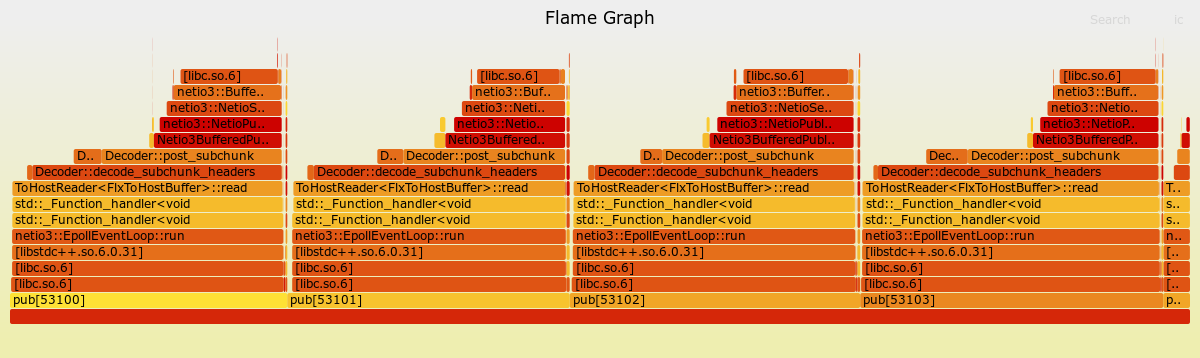
\includegraphics[width=\textwidth]{images/results/flamegraph.png}
\caption[Flamegraph of felix-tohost]{Flamegraph of \texttt{felix-tohost}. It highlights four main processes, each corresponding to one \acs{DMA} buffer, along with a smaller fifth process dedicated to \acs{TTC}.}\label{fig:felix-tohost-flamegraph}
\end{figure}